\section{Race conditions in web applications}

Modern web applications rely on concurrency in order to serve multiple users at the same time. Different web servers employ different concurrency techniques, but they all achieve the same result of being able to process multiple requests in parallel. This makes web applications particularly susceptible to race conditions. \\

The previous example shows that this must be carefully taken into consideration when dealing with databases, which web applications often use to store persistent data. The \texttt{aart} challenge is yet another example (certainly the most realistic so far) where this principle is not honored.

\subsection{\texttt{aart} challenge walkthrough}

The challenge presents itself as a simple web application that allows users to register, login and share and vote ASCII art. The server-side source code is given and reveals that the application is written in PHP and uses a MySQL database for persistent data storage. \\

\subsubsection{Vulnerability}
 
A good first approach for assessing vulnerabilities in the web application is to try and use it as intended, looking for unexpected behaviours or error messages. While registration of a new user account works with no particularities, attempting to login results in a message warning that our account is restricted.

\begin{figure}[h]
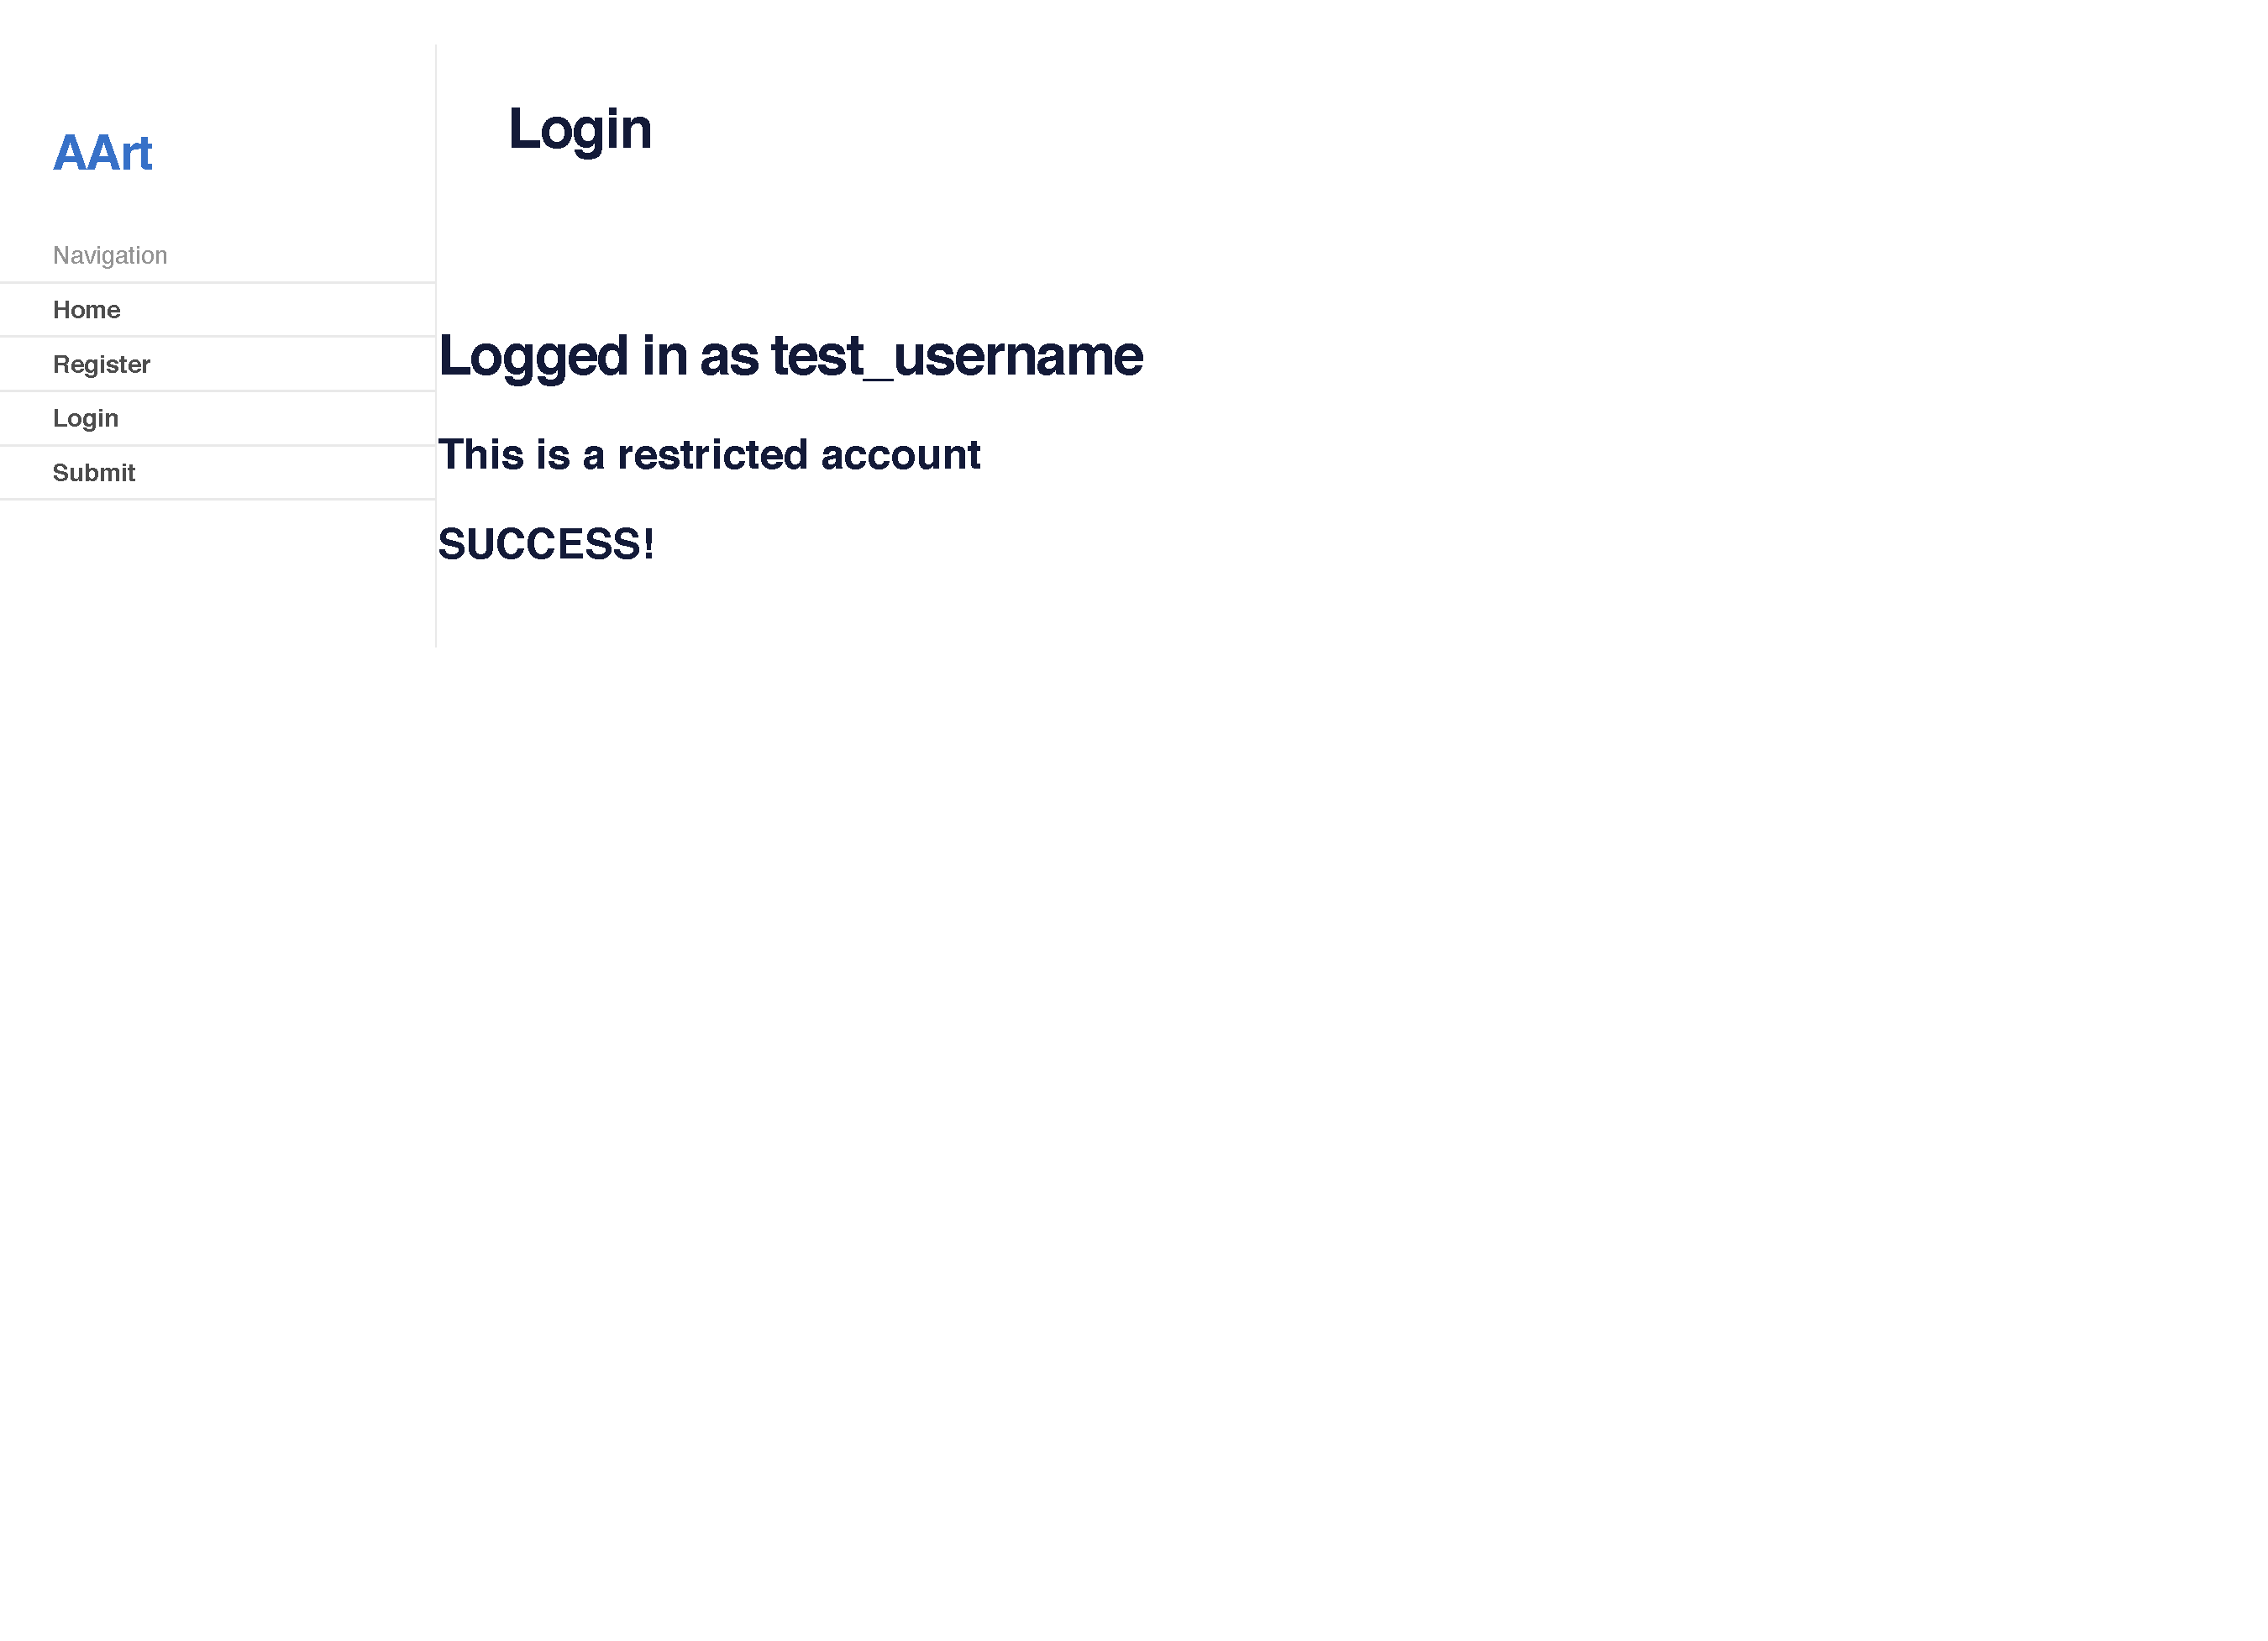
\includegraphics[width=\textwidth]{img/aart_login.pdf}
\caption{Post-login page of the \texttt{aart} web application}
\label{fig:aartlogin}
\end{figure}

The message can be investigated by searching it through the source code of the application. The only occurrence is in file \texttt{login.php} file, of which the relevant part is reported in Listing~\ref{listing:login}.

\begin{listing}[H]
\newenvironment{whitetext}{\par\color{white}}{\par}
\begin{whitetext}
\renewcommand{\theFancyVerbLine}{\rmfamily\textcolor{black}{\tiny{\arabic{FancyVerbLine}}}}
\begin{minted}[escapeinside=!!, firstline=2, lastline=16, firstnumber=27, breaklines]{html+php}
<?php
$uid = $row['id'];
$sql = "SELECT isRestricted from privs where userid='$uid' and isRestricted=TRUE;";
$result = mysqli_query($conn, $sql); !\label{permcheck}!
$row = $result->fetch_assoc(); !\label{fetchassoc}!
if($row['isRestricted']){
    ?>
    <h2>This is a restricted account</h2> !\label{errormsg}!

    <?php
}else{
    ?>
    <h2><?php include('../key');?></h2> !\label{flag}!
    <?php

}
?>
\end{minted}
\end{whitetext}
\caption{Extract from file \texttt{login.php}}
\label{listing:login}
\end{listing}

The code queries the database in order to check whether the \texttt{privs} table has a \texttt{isRestricted} flag set to true for the current user. If it does, the error message is shown (line~\ref{errormsg}). Otherwise, a file called \texttt{key} is included in the page (line~\ref{flag}). \\

It is reasonable to guess that the \texttt{key} file -- which is not included among the source code of the application -- contains the flag, thus our objective becomes to login with an account which does not have the \texttt{isRestricted} flag set to true\footnote{Notice that having the \texttt{isRestricted} flag set to false is not necessary; having no row at all associated with the current user in the \texttt{privs} table works as well. In that case, \texttt{\$row} at line~\ref{fetchassoc} will have value \texttt{NULL}, thus at the next line \texttt{\$row[\textquotesingle isRestricted\textquotesingle ]} will also be \texttt{NULL}, which evaluates to \texttt{false}. A simple null check or using a strict comparison (e.g. \texttt{if~(\$row[\textquotesingle isRestricted\textquotesingle ]~===~false)}) would have made the objective much harder or impossible to achieve.}. \\

By searching again through the code, it is possible to discover that the value \texttt{isRestricted} also appears in \texttt{register.php} file.

\begin{listing}[H]
\begin{minted}[escapeinside=!!, startinline, firstnumber=13, breaklines]{php}
$username = mysqli_real_escape_string($conn, $_POST['username']);
$password = mysqli_real_escape_string($conn, $_POST['password']);

$sql = "INSERT into users (username, password) values ('$username', '$password');"; !\label{query1}!

mysqli_query($conn, $sql); !\label{exec1}!
$sql = "INSERT into privs (userid, isRestricted) values ((select users.id from users where username='$username'), TRUE);"; !\label{query2}!
mysqli_query($conn, $sql); !\label{exec2}!
\end{minted}
\caption{Extract from file \texttt{register.php}}
\end{listing}

Here two queries are prepared and executed. The first one, at line~\ref{query1}, performs the user registration by inserting the corresponding row into the database. The second one, at line~\ref{query2}, inserts a row into the \texttt{privs} table with the \texttt{isRestricted} flag set to true for the newly registered user. This second query is the reason why any user that registers on the application will see the message shown in Figure~\ref{fig:aartlogin} upon login. \\

Notice that the two queries are executed independently of each other. Once again, there is no use of database transactions and this leads to a race condition vulnerability. With accurate timing, an attacker could log into the application after the first query is executed but before the second query is, i.e.  during the (short) period of time that occurs between lines \ref{exec1} and \ref{exec2}, where the user is registered but it is not restricted yet. \\

\subsubsection{Exploit}

The easiest way of exploiting this vulnerability is to repeatedly make two almost simultaneous requests -- one for registration and one for login -- until the second request happens to be processed while the execution of the first one has reached the \textit{sweet spot} described before.

\begin{table}[H]
\centering
\begin{tabular}{|l|l|}
\hline
\thead[c]{\textbf{\texttt{register.php} request}} & \thead[c]{\textbf{\texttt{login.php} request}} \\ \hline
\makecell[tl]{Registration query (line~\ref{exec1})} & \\
& \makecell[tl]{Login query (credentials check)} \\
& \makecell[tl]{\textcolor{red}{Permissions check query (line~\ref{permcheck})}}  \\
\makecell[tl]{Permissions update query (line~\ref{exec2})} &  \\  \hline
\end{tabular}
\caption{Execution order required for exploiting the vulnerability}
\label{tab:exploit}
\end{table}

For this purpose, we can write a Python script and use the \texttt{threading} module to make concurrent requests. \\

\begin{listing}[h]
\inputminted[python3]{python}{code/aart.py}
\caption{Script used to exploit the race condition vulnerability in \texttt{aart}}
\label{listing:exploit}
\end{listing}

The script in Listing~\ref{listing:exploit} attempts to exploit the vulnerability by starting two threads one immediately after the other. The first one performs the registration, while the second one performs the login and checks if the flag is present on the page returned by the server. \\

Since there are no guarantees that the second thread will perform the login at the exact correct time, we repeat the process in a \texttt{while} loop until it succeeds. In any case, empirical tests for this specific case show that exploiting the vulnerability does not usually require more than a couple loops.
